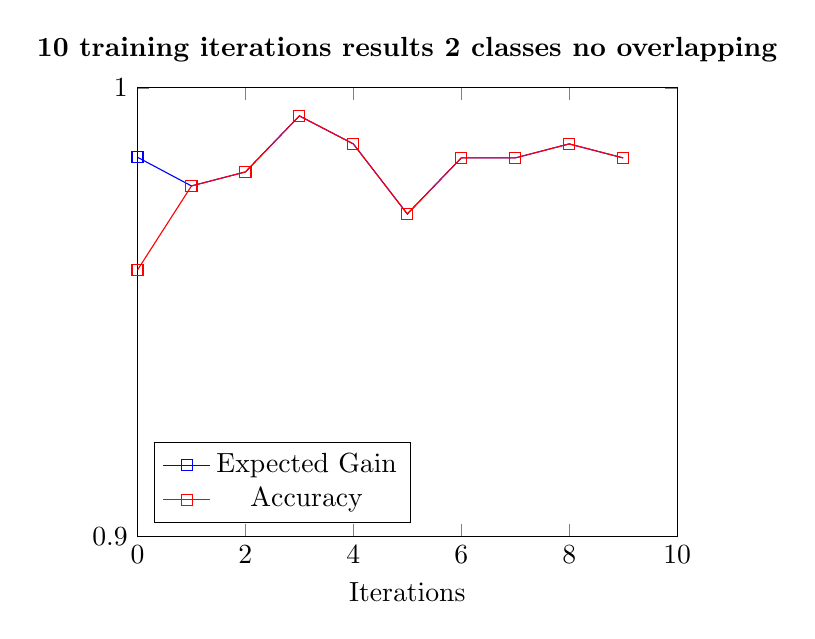
\begin{tikzpicture}
  \begin{axis}[
      title=\textbf{10 training iterations results 2 classes no overlapping},
      xlabel={Iterations},
      xmin=0, xmax=10,
      ymin=0.9, ymax=1,
      xtick={0,2,4,6,8,10},
      ytick={0.9,1.0},
      legend pos=south west,
      ymajorgrids=true,
      grid style=dashed,
  ]
  
  \addplot[color=blue, mark=square]
    coordinates {
      (0,0.9845253073815597)
      (1,0.9781249999999999)
      (2,0.98125)
      (3,0.9937500000000001)
      (4,0.9875000000000002)
      (5,0.971875)
      (6,0.9843750000000001)
      (7,0.9843750000000001)
      (8,0.9875000000000002)
      (9,0.9843750000000001)
    };
    \addlegendentry{Expected Gain}
  
  \addplot[color=red, mark=square]
    coordinates {
      (0,0.959375)
      (1,0.978125)
      (2,0.98125)
      (3,0.99375)
      (4,0.9875)
      (5,0.971875)
      (6,0.984375)
      (7,0.984375)
      (8,0.9875)
      (9,0.984375)
    };
    \addlegendentry{Accuracy}
      
  \end{axis}
\end{tikzpicture}